\documentclass[aspectratio=169]{beamer}
\usetheme{metropolis}

\usepackage[utf8]{inputenc}
\usepackage[T1]{fontenc}
\usepackage{booktabs}
\usepackage{multicol}
\usepackage{graphicx}
\usepackage{tikz}
\usepackage{xcolor}

\graphicspath{{../images/}}

\definecolor{papertitle}{HTML}{C45911}
\definecolor{venue}{HTML}{7BA4CC}
\newcommand{\paper}[3]{\textcolor{papertitle}{#1} {\footnotesize\textcolor{venue}{#2}} {\footnotesize #3}}

\title{ChRiGiD: Engineering of Data Analysis Pipelines}
\subtitle{ERC CZ Grant LL2325}
\author{Jan Vitek}
\institute{Faculty of Mathematics and Physics\\Charles University, Prague}
\date{2026}

\begin{document}

%% ---- Title Slide ----
{
\usebackgroundtemplate{%
  \tikz[overlay,remember picture]
    \node[opacity=0.3,at=(current page.center)] {%
      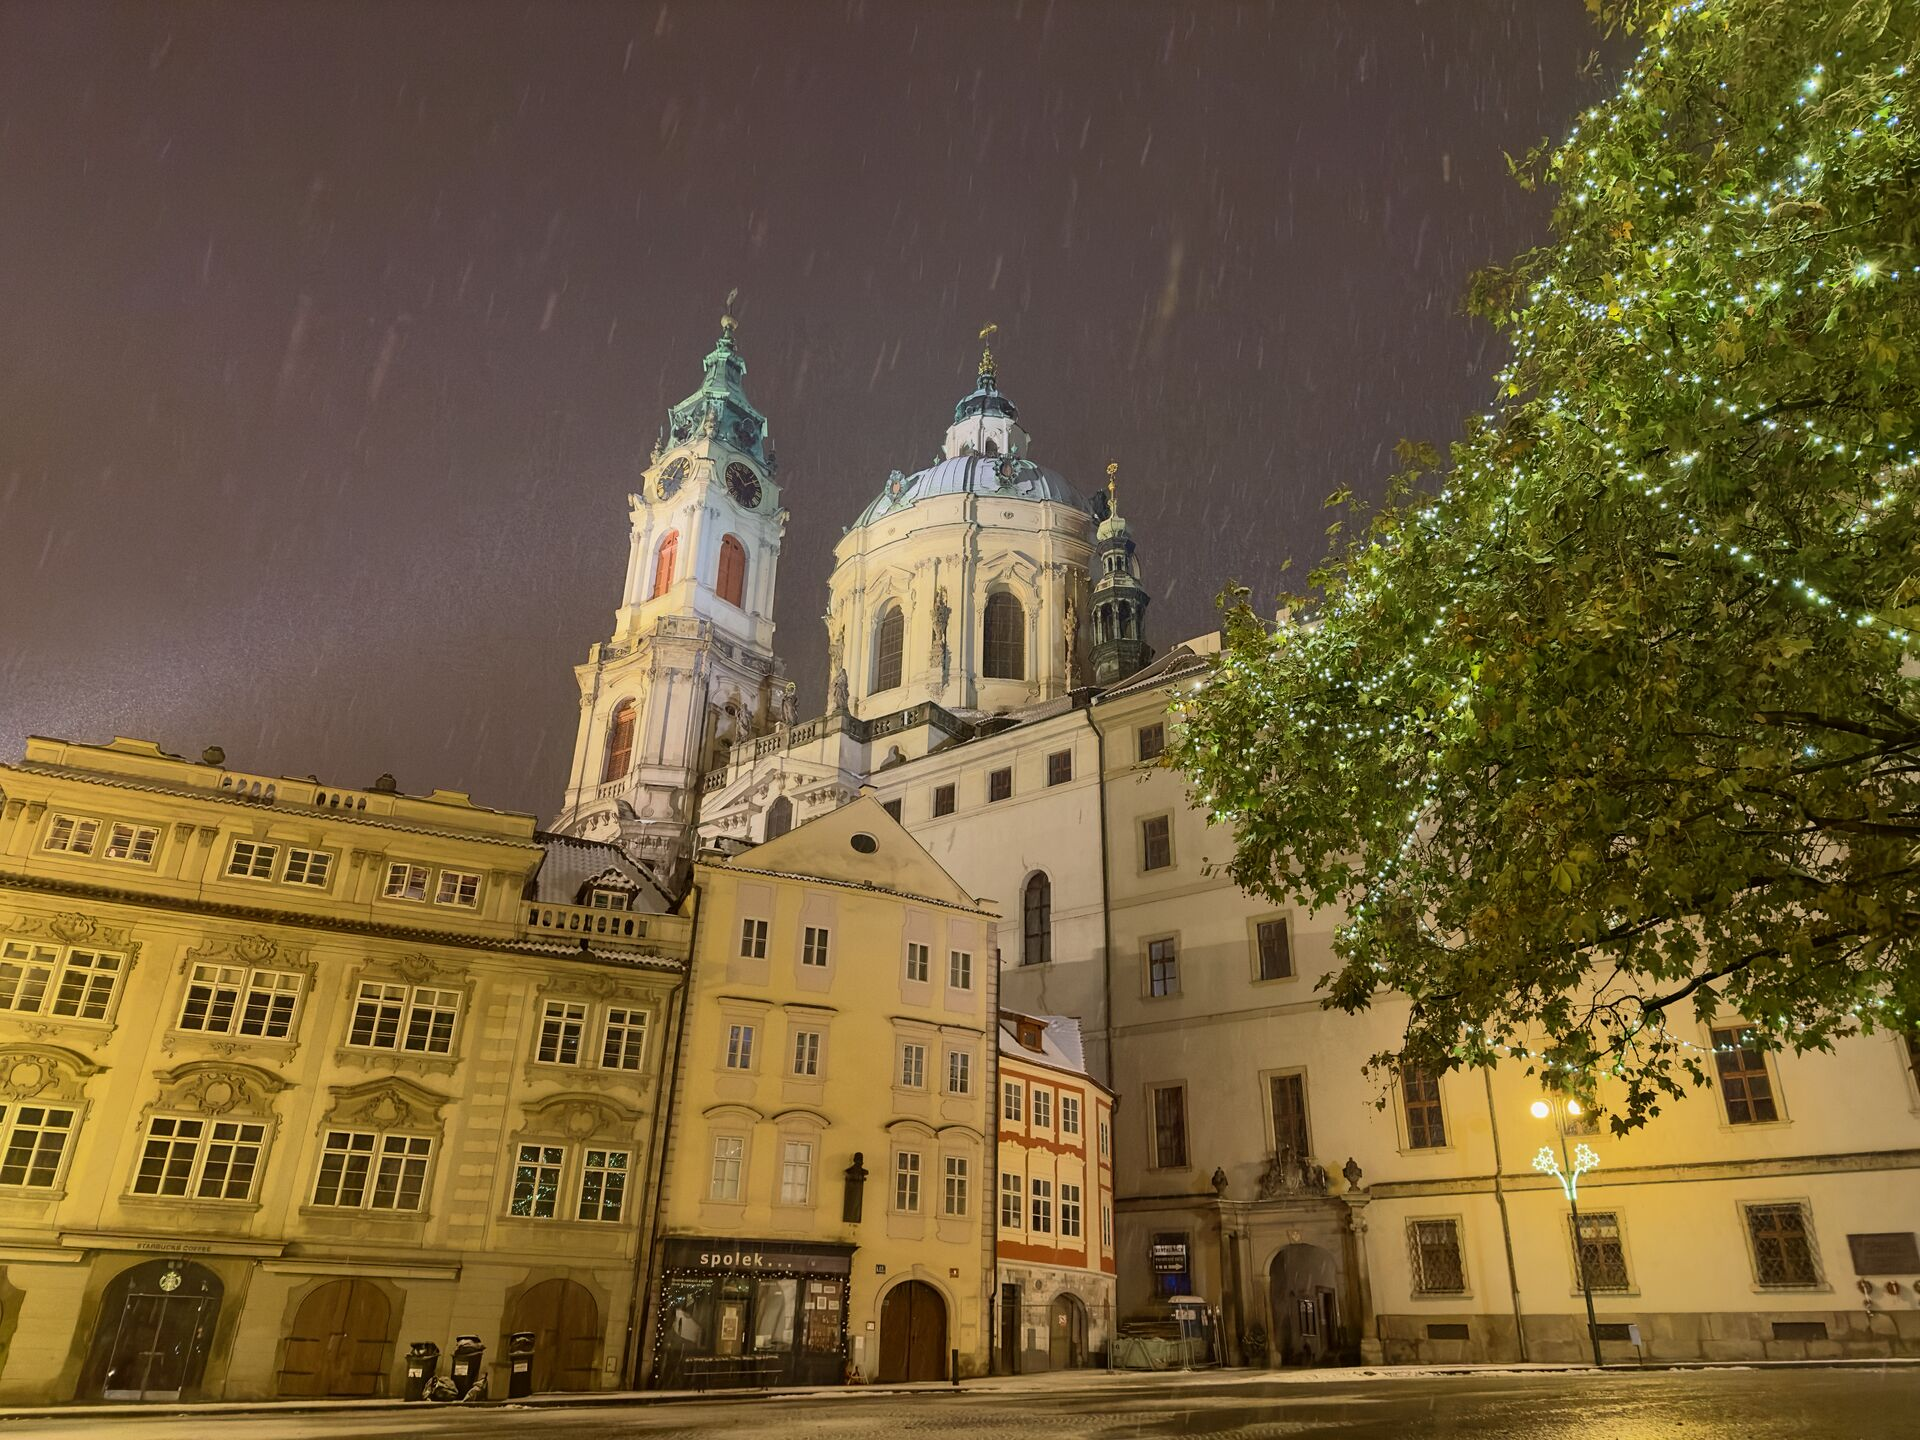
\includegraphics[width=\paperwidth]{IMG_2303.jpg}};
}
\begin{frame}
  \maketitle
  \vfill
  \centering
  \begin{minipage}{0.8\textwidth}
    \centering
    
\includegraphics[height=1cm]{logo/erc_logo_inv.png}\hspace{1.5em}%
    
\includegraphics[height=1cm]{logo/msmt-logo-no-backgroung.png}\hspace{1.5em}%
    
\includegraphics[height=1cm]{logo/eu_flag_round-nobg.png}\hspace{1.5em}%
    
\includegraphics[height=1cm]{logo/PR-56-version1-uk_slavnostni_eng_barevna.png}
  \end{minipage}
\end{frame}
}

%% ---- Research Themes ----
\begin{frame}{Research Themes}
  \begin{description}
    \item[Practical Data Science]
      Understanding how data scientists work and where things go wrong
      through user studies, interviews, and large-scale analysis of real-world code.

    \medskip
    \item[Type Systems]
      Developing type systems that catch errors in dynamic languages
      without getting in the way---gradual typing, set-theoretic types,
      and type inference.

    \medskip
    \item[Tools and Languages]
      Building compilers, runtime systems, and development tools---JIT
      compilation, automated test generation, reproducibility, and data
      lineage tracking.
  \end{description}
\end{frame}

%% ---- Highlights ----
\begin{frame}{2023--2025 Highlights}
  \begin{itemize}
    \item 14 peer-reviewed publications
    \item 4 open-source software artifacts
    \item 11-member international team
    \item Selected to host \textbf{SPLASH 2027} --- first time in Central Europe (${\sim}$\$1M budget, 400--500 attendees)
    \item Organized \textbf{PLISS 2025} summer school (Bertinoro, Italy; with King's College, \v{C}VUT, Northeastern)
    \item Launched joint \textbf{UK--\v{C}VUT research meetings} on programming languages
    \item \textbf{HORIZON FRITES} EU Pathfinder Open proposal with CNRS, TU Kaiserslautern, Ericsson, et al.\ (not funded; will resubmit)
    \item Visiting researchers: Noller (Ruhr U.\ Bochum), Thakur (IIT), Sihler (Ulm U.)
  \end{itemize}
\end{frame}

%% ---- Team ----
\newcommand{\teamphoto}[2]{%
  \begin{minipage}{0.18\textwidth}\centering
    \includegraphics[width=1.6cm,height=1.6cm,keepaspectratio]{people/#1}\\[-2pt]
    {\scriptsize #2}
  \end{minipage}%
}

\begin{frame}{Staff}
  \centering
  \smallskip
  \teamphoto{jan_vitek.jpg}{Vitek (PI)}
  \teamphoto{jan_kofron.png}{Kofro\v{n}}
  \teamphoto{pavel_parizek.png}{Par\'izek}
  \teamphoto{tomas_petricek.png}{Pet\v{r}\'i\v{c}ek}
  \teamphoto{robert_grimm.jpg}{Grimm}

  \medskip
  \teamphoto{joel_jakubovic.png}{Jakubovic}
  \teamphoto{mickael_laurent.jpg}{Laurent}
  \teamphoto{jakob_hain.jpg}{Hain}
  \teamphoto{placeholder_1.png}{Kocourek}
  \teamphoto{placeholder_2.png}{Skotorenko}

  \medskip
  \teamphoto{lucie_lerch.jpg}{Lerch}

  \vfill
  \small\textit{Alumni:} Boruch-Gruszecki, Blicha, Je\v{z}ek, Sihler
\end{frame}

%% ---- Publications ----
\begin{frame}{Publications --- 2024}
  \small
  \begin{enumerate}
    \item \paper{Data Lineage Analysis for Enterprise Applications by Manta}{ICSE-SEIP}{Par\'izek, Hermann}
    \item \paper{Decidable Subtyping of Existential Types for Julia}{PLDI}{Belyakova, Chung, Tate, Vitek}
    \item \paper{Gradient: Gradual Compartmentalization via Capabilities}{OOPSLA}{Boruch-Gruszecki et al.}
    \item \paper{Pure Methods for roDOT}{ECOOP}{Dort, Li, Lho\'tak, Par\'izek}
    \item \paper{Reducing Feedback Pollution}{VMIL}{Krynski, \v{S}t\v{e}p\'anek, \v{R}\'iha, K\v{r}ikava, Vitek}
    \item \paper{The Fault in Our Stars}{ECOOP}{Maj, Muroya, Siek, Di Grazia, Vitek}
  \end{enumerate}
\end{frame}

\begin{frame}{Publications --- 2025}
  \small
  \begin{enumerate}
    \item \paper{Combining Static Analysis Techniques for Program Comprehension Using Slicito}{ICPC}{Husak, Kofro\v{n}, Zavoral}
    \item \paper{Copy-and-Patch Just-in-Time Compiler for R}{VMIL}{Kocourek, K\v{r}ikava, Vitek}
    \item \paper{Denicek: Computational Substrate for Document-Oriented End-User Programming}{UIST}{Pet\v{r}\'i\v{c}ek, Edwards}
    \item \paper{Ethics of Sentiment Analysis and Theology}{HTS}{Je\v{z}ek}
    \item \paper{Locating Concurrency Errors in Windows .NET Applications}{SPIN}{Kliber, Par\'izek}
    \item \paper{R4R: Reproducibility for R}{ACM REP}{Donat-Bouillud, K\v{r}ikava, Krynski, Vitek}
    \item \paper{The Unix Executable as a Smalltalk Method}{Onward!}{Jakubovic}
    \item \paper{Toward a Typed Intermediate Language for R}{Programming}{Laurent, Hain, Krikava, Krynski, Vitek}
  \end{enumerate}
\end{frame}


%% ---- Software ----
\begin{frame}{Open-Source Software}
  \begin{description}
    \item[Shantay] EU DSA Transparency Database processing tool (Apache 2.0)
    \item[Denicek] Computational substrate for document-oriented end-user programming (MIT)
    \item[R Bytecode Compilers] Bytecode compiler for R in Rust and Java for performance comparison (GPL-3.0 / MIT)
    \item[Smalltix] Smalltalk VM via filesystem, identifying Unix executables with Smalltalk methods (Unlicense)
  \end{description}
\end{frame}

\end{document}
